%!TEX root = ../main.tex
% Chapter Template

\chapter{Introduction to Machine Learning} % Main chapter title

\label{Chapter2} % Change X to a consecutive number; for referencing this chapter elsewhere, use \ref{ChapterX}

%----------------------------------------------------------------------------------------
%	SECTION 1
%----------------------------------------------------------------------------------------

\section{Machine Learning Basics}

Deep learning is a specific kind of machine learning. To understand deep learning well, one must have a solid understanding of machine learning. Machine learning is a form of applied statistics with an increased emphasis on the use of computers to statistically estimate complicated functions and a decreased emphasis on proving confidence intervals around these functions.

\parencite{machine-learning} describes a machine learning a task as: "A computer program is said to learn from experience \(E\) with respect to some class of tasks \(T\) and performance measure \(P\), if its performance at tasks in \(T\), as measured by \(P\), improves with experience \(E\)."

%-----------------------------------
%	SUBSECTION 1
%-----------------------------------
\subsection{The task \(T\)}

In this definition of "task", the process of learning itself is not the task. For example, if we want a program to learn to distinguish dogs and cats, then distinguishing dogs and cats is the task.

Machine learning tasks are usually described in terms of how the machine learning system should process an example. An example is a collection of features that have been quantitatively measured from some object or event that we want the machine learning system to process. We typically represent an example as a vector \(x \in \RR^n\) where each entry \(x_i\) of the vector is a feature. For example, the features of an image are usually the values of the pixels in the image. Some tipical examples of tasks are:

\begin{itemize}
    \item \textbf{Classification}: Classification tasks ask the computer program to specify in which category does one input vector belong. Formally, this is equivalent to approximate a function \(f:\RR^n \mapsto \{1, 2, \ldots, k\}\).
    \item \textbf{Regression}: In this type of task, the computer program is asked to predict a numerical value given some input. This consists in approximating a function \(f:\RR^n \mapsto \RR\).
    \item \textbf{Transcription}: In this type of task, the machine learning system is asked to observe an unstructured representation of some kind of data and transcribe the information into text. For example, in optical character recognition (OCR), the computer program is shown an image containing text and is asked to return this text in the form of a sequence of characters.
    \item \textbf{Denoising}: In this type of task, the machine learning algorithm is given an input a corrupted example \(\tilde{x} \in \RR^n\) obtained by an unknown corruption process from a clean example \(x \in \RR^n\).
\end{itemize}

%-----------------------------------
%	SUBSECTION 2
%-----------------------------------

\subsection{The Performance Measure, \(P\)}
To evaluate how good our machine learning algorithm is, we must desing quantitatives measures of its performance. For tasks such as classification, we often measure the \textbf{accuracy} of the model, which is just the proportion of examples for which the algorithm gives the correct output. (similarly, the \textbf{error rate} is the p{}roportion of examples for which the algorithm gives an incorrect output).

Usually, we are interested in seeing how well an algorithm performs on data it has not seen before, since this will determine how well it will work "in the real world". To determine this, we usually evaluate \(P\) using a \textbf{test set} of our data, which we have previously split from the \textbf{train set}

%-----------------------------------
%   SUBSECTION 3
%-----------------------------------

\subsection{The Experience, \(E\)}
Machine learning algorithms can be understood as beaing allowed to experience an entire \textbf{dataset}. A dataset is a collection of many \textbf{examples}.

Generally, machine learning algorithms can be categorized as \textbf{supervised} or \textbf{unsupervised}
\begin{itemize}
\item \textbf{Unsupervised}: The algorithm experiences a dataset containing features and has to learn some structure or pattern from it.
\item \textbf{Supervised}: The algorithm experiences a dataset containing features, but each example is algo associated with a \textbf{label} of \textbf{target}. We will generally refer the examples as \(\bm{x}\) and to the targets as \(\bm{y}\). When we talk about a specific example and target, we will use superindeces: \(\bm{x}^{(i)}\) and \(\bm{y}^{(i)}\)

\end{itemize}
Throughout this work, we will focus mainly on supervised learning, i. e. each example has \(\bm{x}^{(i)}\) a corresponding target \(\bm{y}^{(i)}\).

Some machine learning algorithms do not just experience a dataset. For example, \textbf{reinforcement learning} algorithms interact with a enviroment, so there is a feedback loop between the algorithm and its experiences. An example of reinforcement learnings algorithm is AlphaGo Zero from Google \parencite{alphago}, an algorithm that learned to play the game of go from scratch better than any human. 


%----------------------------------------------------------------------------------------
%	SECTION 2
%----------------------------------------------------------------------------------------

\section{Capacity, Overfitting and Underfitting}

The central challenge of machine learning is that our algorithm must perform well on unseen examples. This is called \textbf{generalization}.

Typically, when training a machine learning model, we compute some error measure over our training set, called \textbf{training error}. This is simply an optimization problem. In machine learning, we want the \textbf{test error}, computed over a text set which the algorithm has never seen to be low as well. The test error will always be greater or equal than the training error.

The factors to determine how well a machine learning algorithm will perform are its ability to make the training error small, and to make the gap between the training error and the test (\textbf{generalization gap}) error small. These two factors correspond to \textbf{underfitting} (when the training error is too high) and \textbf{overfitting} (when the generalization gap is too high).

Wether a model is going to underfit or overfit depends on its \textbf{capacity}, which correspond to the capability of a model to approximate a wide variety of functions. Models with low capacity cannot fit the training set. Models with high capacity will overfit the training set, and the generalization gap will be large.

\begin{figure}
    \centering
    \begin{subfigure}[b]{0.3\textwidth}
        \centering
        \caption{Underfitting}
        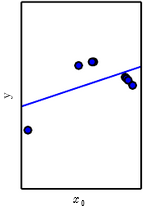
\includegraphics[width=\textwidth]{Figures/underfit}
        \label{fig:y equals x}
    \end{subfigure}
    \hfill
    \begin{subfigure}[b]{0.3\textwidth}
        \centering
        \caption{Appropiate capacity}
        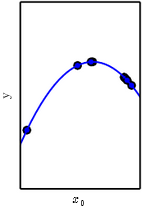
\includegraphics[width=\textwidth]{Figures/appropiate}
        \label{fig:three sin x}
    \end{subfigure}
    \hfill
    \begin{subfigure}[b]{0.3\textwidth}
        \centering
        \caption{Overfitting}
        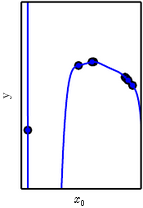
\includegraphics[width=\textwidth]{Figures/overfit}
        \label{fig:five over x}
    \end{subfigure}
    \decoRule
    \caption[Underfitting and overfitting]{Here we have three examples of a regression. The training data was generated synthetically, by randomly sampling \(x\) values and choosing \(y\) deterministically by evaluating a quadratic function. (A) A linear function cannot capture the curvature and underfits the data. (B) A quadratic function fits to the data and generalizes well to unseen points. It does not suffer from overfitting or underfitting. (C) A polynomial of degree 9 overfits the data and does not generalize well to unseen points \parencite{deep-learning}.}
    \label{fig:overfit}
\end{figure}

%-----------------------------------
%   SUBSECTION 1
%-----------------------------------
\subsection{Regularization}

Regularization is a technique to avoid overfitting, and thus reduce the generalization gap. For example, in figure \ref{fig:overfit}, we could "penalize" our algorithm for having large parameters. This would reduce the algorithm capacity (it would increase the training error), but it would help avoid overfitting (decreasing the generalization gap).

There are many ways to \textbf{regularize}, and which is the correct way depends on the task we want our algorithm to solve.

%-----------------------------------
%   SUBSECTION 2
%-----------------------------------
\subsection{The No Free Lunch Theorem}

The no free lunch theorem \parencite{no-free-lunch} says that, averaged over all possible data, every classification algorithm has the same error rate when classifying previously unobserved points. This means that no machine learning algorithm is better than any other in all possible tasks. 

Fortunately, this results only holds when we average over all data-generating distributions. This means that if we make assumptions about the distributions that we will find in the real world, we can design an algorithm that does well in these distributions.

The no free lunch theorem implies that we must design our algorithm to work well only on a single task. This is done by assuming building hypothesis into the algorithm. For example, in a linear regression will work well if the outputs come from a linear function applied to the inputs, but will not work if the thata is of the form \(y=sin(x)\).

%----------------------------------------------------------------------------------------
%   SECTION 3
%----------------------------------------------------------------------------------------

\section{Gradient-Based Optimization}

Many machine learning algorithms and nearly all deep learning algorithms use \textbf{Stochastic Gradient Descent} (\textbf{SGD}), which is an extension from the classical Gradient Descent. 

%-----------------------------------
%   SUBSECTION 1
%-----------------------------------
\subsection{Gradient Descent}

Generally, for an algorithm to learn a task it has to optimize some \textbf{objective function} or \textbf{loss function}. In general, this function will be a measure of the error, and we will want to minimize it with respect the parameters of our algorithm.

It is well known that the gradient of a function gives the direction of maximum ascend, so, for small enough \(\epsilon\), \(f(\bm{x} - \epsilon\nabla f(\bm{x}))\) will be smaller than \(f(\bm{x})\). We can iterate this process, which will reduce \(f(\bm{x})\) at each step. This technique is called fgradient descent \parencite{cauchy1847methode}.

In machine learning, the \(\epsilon\) parameter is called learning rate, as it symbolizes the speed at which the algorithm learns. Choosing the right learning rate is crucial, since a learning rate too low will make the algorithm learn too slowly, and a learning rate to high will make the gradient descent diverge and not find a minimum.

If \(L\) is the loss function that we want to minimize with respect to some parameters \(\bm{\theta}\), and \(\bm{x}\) and \(\bm{y}\) are the examples with their corresponding labels, and \(\bm{f}\) is the function that we are approximating, the update rule will be:

\begin{equation}
\bm{\theta} \leftarrow \bm{\theta} - \epsilon \nabla_{\bm{\theta}} L\left(\bm{f}(\bm{x};\bm{\theta}),\bm{y}\right)
\end{equation}

%-----------------------------------
%   SUBSECTION 2
%-----------------------------------
\subsection{Stochastic Gradient Descent}

A problem in machine learning is that large datasets give better results, but they are algo computiationally expensive.

Usually, the loss function in a machine learning algorithm decomposes in the sum of some per-example loss function:

\begin{equation}
L_{\text{total}}\left(\bm{f}(\bm{x};\bm{\theta}),\bm{y}\right) = \frac{1}{m}\sum_{i=1}^m L\left(\bm{f}(\bm{x}^{(i)};\bm{\theta}),\bm{y}^{(i)}\right)
\end{equation}

 If the training examples grows to billions, the cost to make a single gradient step becomes too large.

The idea behind SGD is that the gradient is just an expected value of the largest descent direction, and it can be estimated with a small set of examples. On each step we can sample a \textbf{minibatch} of examples \(\mathbb{B}=\{\bm{x}^{(1)}, \bm{x}^{(2)}, \ldots,  \bm{x}^{(m')\}}\) from the whole dataset, and estimate \(\nabla f(x)\) using only these examples. The idea is that \(m'\) is fixed even though the size of the dataset can grow.
\begin{equation}
\nabla_{\bm{\theta}}L_{\text{total}}\left(\bm{f}(\bm{x};\bm{\theta}),\bm{y}\right) \approx \nabla_{\bm{\theta}}\frac{1}{m'}\sum_{i=1}^{m'} L\left(\bm{f}(\bm{x}^{(i)};\bm{\theta}),\bm{y}^{(i)}\right)
\end{equation}

%-----------------------------------
%   SUBSECTION 3
%-----------------------------------
\subsection{Momentum}

Even though SGD works well, it can sometimes be slow. The method of momentum is designed to accelerate learning, especially in the face of high curvature, small but consistent gradients or noisy gradients.

The momentum algorithm introduces a variable \(v\) that plays the role of velocity. The name momentum derives from the physical analogy. The new update rule is given by:

\begin{align}
\bm{v} &\leftarrow \alpha \bm{v} - \epsilon \nabla_{\bm{\theta}}\frac{1}{m'}\sum_{i=1}^{m'} L\left(\bm{f}(\bm{x^{(i)}};\bm{\theta}),\bm{y^{(i)}}\right)\\
\bm{\theta} &\leftarrow \bm{\theta} + \bm{v}
\end{align}

Here, \(\alpha\) determines how quickly the contribution from previous gradients decays.

\begin{figure}[th]
\centering
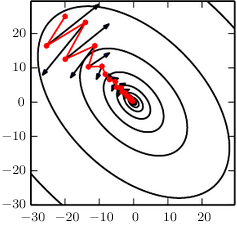
\includegraphics{Figures/momentum}
\decoRule
\caption[Momentum]{Here we can see that the steps (in red) that the momentum takes go in the direction of the minimum, while the gradient (in black) points in other direcitons \parencite{deep-learning}.}
\label{fig:momentum}
\end{figure}